\documentclass{standalone}
\usepackage{tikz}
\usetikzlibrary{patterns, positioning}
\usepackage[sfdefault]{ClearSans} %% option 'sfdefault' activates Clear Sans as the default text font
\usepackage[T1]{fontenc}

\begin{document}
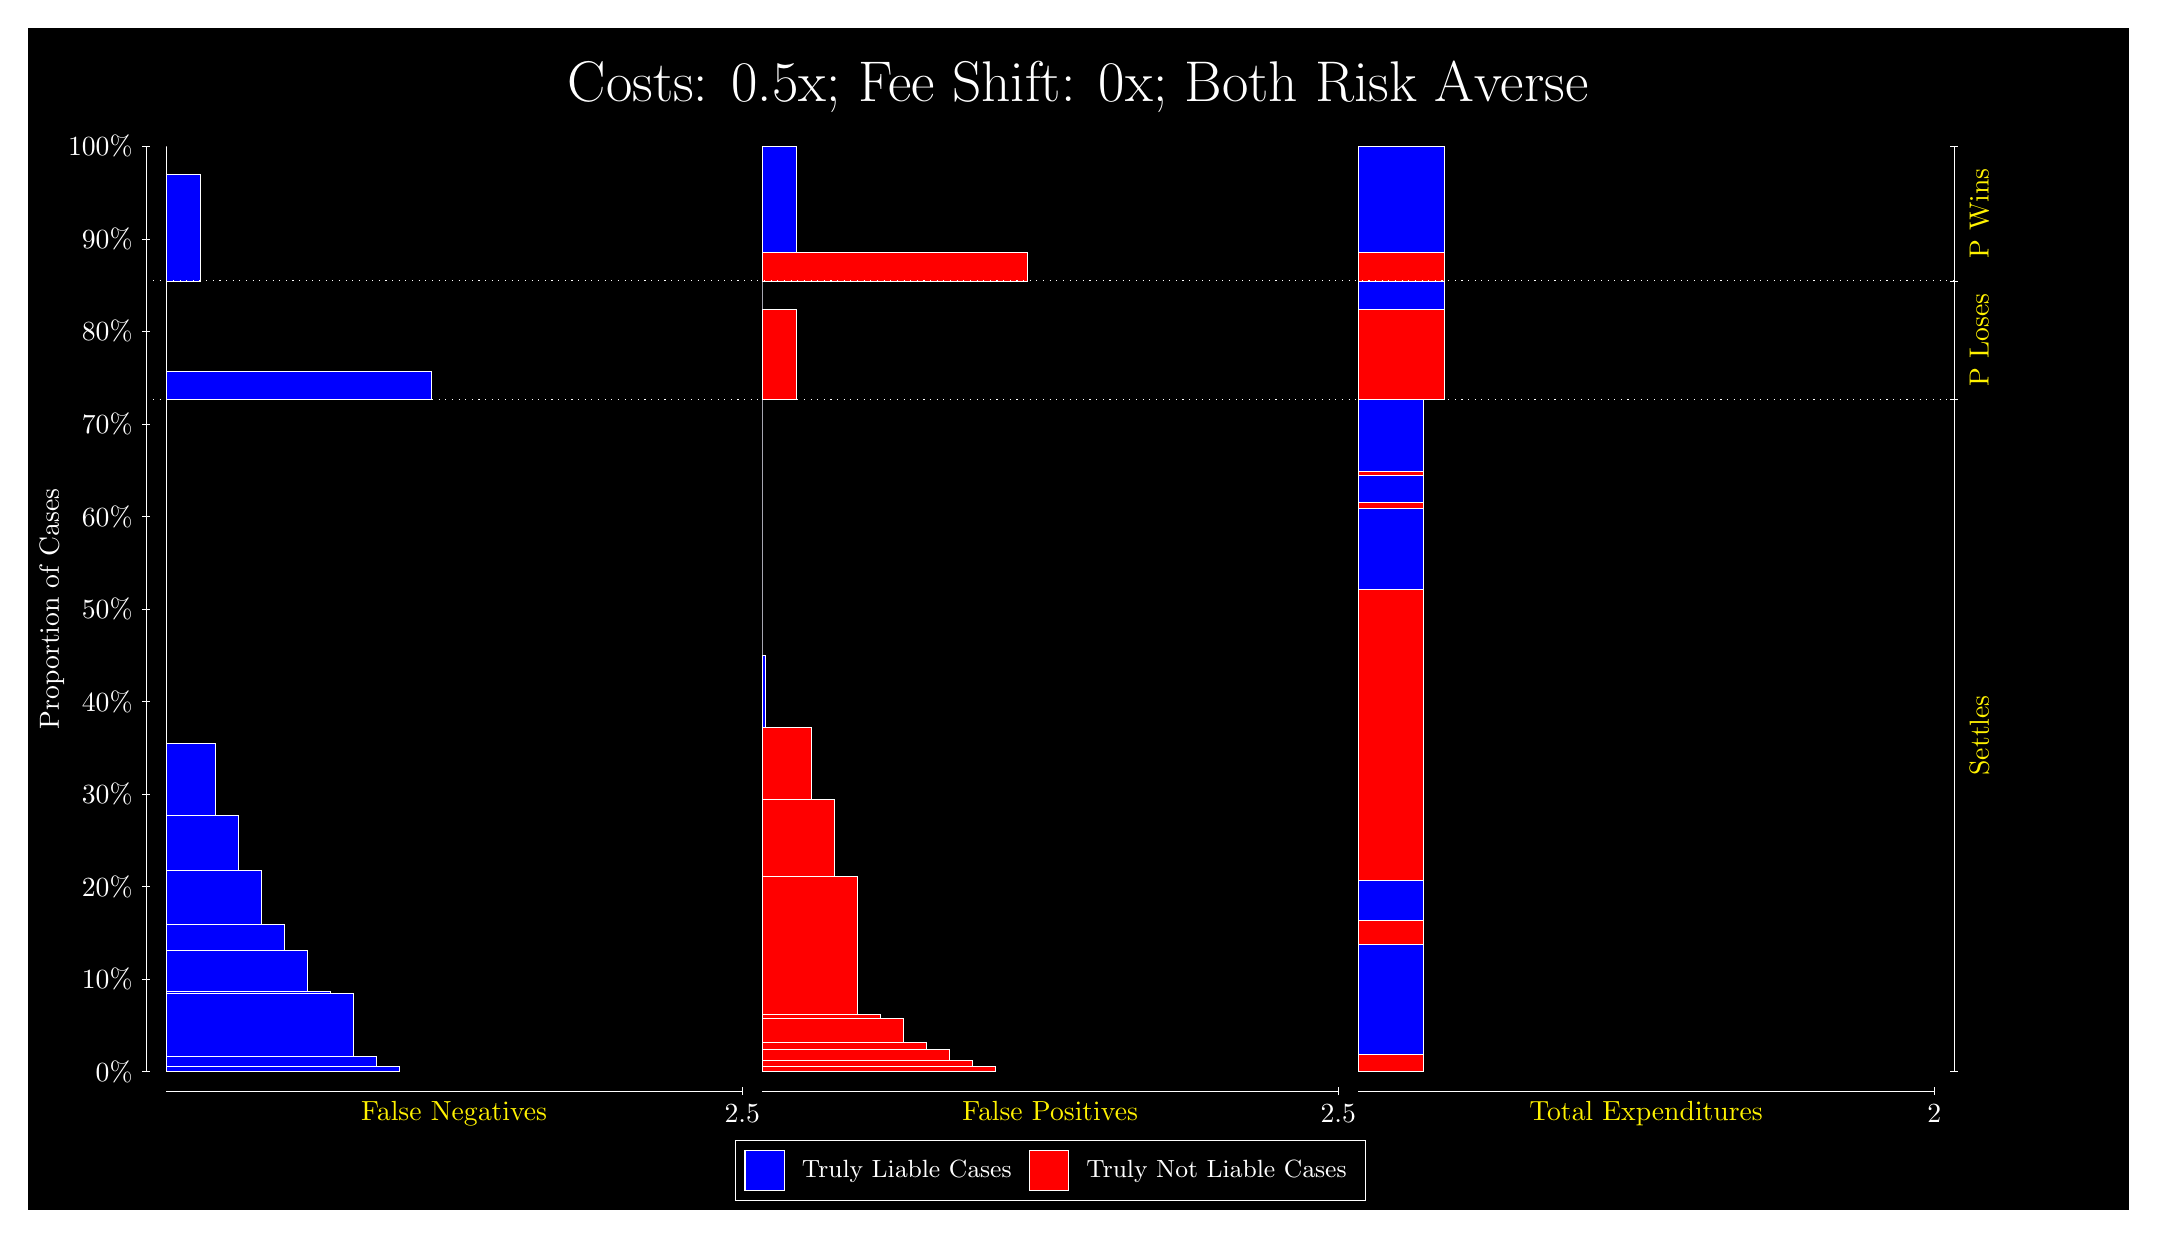
\begin{tikzpicture}
\draw[fill=black] (0,0) rectangle (26.667,15);
\draw[text=white] (0,13.5) rectangle (26.667,15) node[midway] {\huge Costs: 0.5x; Fee Shift: 0x; Both Risk Averse};
\draw[white, very thin] (1.5,1.75) -- (1.5,13.5);
\node[rotate=90, text=white, anchor=center] at (0.3, 7.625) {Proportion of Cases};
\draw[white, very thin] (1.45,1.75) -- (1.55,1.75);
\node[text=white, anchor=east] at (1.45, 1.75) {0\%};
\draw[white, very thin] (1.45,2.925) -- (1.55,2.925);
\node[text=white, anchor=east] at (1.45, 2.925) {10\%};
\draw[white, very thin] (1.45,4.1) -- (1.55,4.1);
\node[text=white, anchor=east] at (1.45, 4.1) {20\%};
\draw[white, very thin] (1.45,5.275) -- (1.55,5.275);
\node[text=white, anchor=east] at (1.45, 5.275) {30\%};
\draw[white, very thin] (1.45,6.45) -- (1.55,6.45);
\node[text=white, anchor=east] at (1.45, 6.45) {40\%};
\draw[white, very thin] (1.45,7.625) -- (1.55,7.625);
\node[text=white, anchor=east] at (1.45, 7.625) {50\%};
\draw[white, very thin] (1.45,8.8) -- (1.55,8.8);
\node[text=white, anchor=east] at (1.45, 8.8) {60\%};
\draw[white, very thin] (1.45,9.975) -- (1.55,9.975);
\node[text=white, anchor=east] at (1.45, 9.975) {70\%};
\draw[white, very thin] (1.45,11.15) -- (1.55,11.15);
\node[text=white, anchor=east] at (1.45, 11.15) {80\%};
\draw[white, very thin] (1.45,12.325) -- (1.55,12.325);
\node[text=white, anchor=east] at (1.45, 12.325) {90\%};
\draw[white, very thin] (1.45,13.5) -- (1.55,13.5);
\node[text=white, anchor=east] at (1.45, 13.5) {100\%};

\draw[white, very thin] (24.457,1.75) -- (24.457,13.5);
\draw[white, very thin] (24.407,1.75) -- (24.507,1.75);
\node[anchor=west] at (24.407, 1.75) {};
\draw[white, very thin] (24.407,10.29) -- (24.507,10.29);
\node[anchor=west] at (24.407, 10.29) {};
\draw[white, very thin] (24.407,11.792) -- (24.507,11.792);
\node[anchor=west] at (24.407, 11.792) {};
\draw[white, very thin] (24.407,13.5) -- (24.507,13.5);
\node[anchor=west] at (24.407, 13.5) {};

\draw[white, very thin, fill=blue] (1.75,1.75) rectangle (4.7141,1.8118);
\draw[white, very thin, fill=blue] (1.75,1.8118) rectangle (4.4214,1.9453);
\draw[white, very thin, fill=blue] (1.75,1.9453) rectangle (4.1286,2.7473);
\draw[white, very thin, fill=blue] (1.75,2.7473) rectangle (3.8359,2.7741);
\draw[white, very thin, fill=blue] (1.75,2.7741) rectangle (3.5431,3.2839);
\draw[white, very thin, fill=blue] (1.75,3.2839) rectangle (3.2504,3.6155);
\draw[white, very thin, fill=blue] (1.75,3.6155) rectangle (2.9576,4.3004);
\draw[white, very thin, fill=blue] (1.75,4.3004) rectangle (2.6649,5.0066);
\draw[white, very thin, fill=blue] (1.75,5.0066) rectangle (2.3721,5.9171);
\draw[white, very thin, fill=red] (1.75,5.9171) rectangle (1.75,10.29);
\draw[white, very thin, fill=blue] (1.75,10.29) rectangle (5.1167,10.649);
\draw[white, very thin, fill=red] (1.75,10.649) rectangle (1.75,11.792);
\draw[white, very thin, fill=blue] (1.75,11.792) rectangle (2.1891,13.14);
\draw[white, very thin, fill=red] (1.75,13.14) rectangle (1.75,13.5);
\draw[white, very thin, fill=red] (9.3189,1.75) rectangle (12.283,1.8118);
\draw[white, very thin, fill=red] (9.3189,1.8118) rectangle (11.99,1.8882);
\draw[white, very thin, fill=red] (9.3189,1.8882) rectangle (11.697,2.0319);
\draw[white, very thin, fill=red] (9.3189,2.0319) rectangle (11.405,2.1158);
\draw[white, very thin, fill=red] (9.3189,2.1158) rectangle (11.112,2.4203);
\draw[white, very thin, fill=red] (9.3189,2.4203) rectangle (10.819,2.4795);
\draw[white, very thin, fill=red] (9.3189,2.4795) rectangle (10.526,4.2333);
\draw[white, very thin, fill=red] (9.3189,4.2333) rectangle (10.234,5.2119);
\draw[white, very thin, fill=red] (9.3189,5.2119) rectangle (9.941,6.1225);
\draw[white, very thin, fill=blue] (9.3189,6.1225) rectangle (9.3555,7.033);
\draw[white, very thin, fill=blue] (9.3189,7.033) rectangle (9.3189,10.29);
\draw[white, very thin, fill=red] (9.3189,10.29) rectangle (9.758,11.432);
\draw[white, very thin, fill=blue] (9.3189,11.432) rectangle (9.3189,11.792);
\draw[white, very thin, fill=red] (9.3189,11.792) rectangle (12.686,12.152);
\draw[white, very thin, fill=blue] (9.3189,12.152) rectangle (9.758,13.5);
\draw[white, very thin, fill=red] (16.888,1.75) rectangle (17.711,1.9701);
\draw[white, very thin, fill=blue] (16.888,1.9701) rectangle (17.711,3.3612);
\draw[white, very thin, fill=red] (16.888,3.3612) rectangle (17.711,3.6656);
\draw[white, very thin, fill=blue] (16.888,3.6656) rectangle (17.711,4.1753);
\draw[white, very thin, fill=red] (16.888,4.1753) rectangle (17.711,7.8776);
\draw[white, very thin, fill=blue] (16.888,7.8776) rectangle (17.711,8.9017);
\draw[white, very thin, fill=red] (16.888,8.9017) rectangle (17.711,8.9857);
\draw[white, very thin, fill=blue] (16.888,8.9857) rectangle (17.711,9.3173);
\draw[white, very thin, fill=red] (16.888,9.3173) rectangle (17.711,9.3791);
\draw[white, very thin, fill=blue] (16.888,9.3791) rectangle (17.711,10.29);
\draw[white, very thin, fill=red] (16.888,10.29) rectangle (17.986,11.432);
\draw[white, very thin, fill=blue] (16.888,11.432) rectangle (17.986,11.792);
\draw[white, very thin, fill=red] (16.888,11.792) rectangle (17.986,12.152);
\draw[white, very thin, fill=blue] (16.888,12.152) rectangle (17.986,13.5);
\draw[white, dotted] (1.5,10.29) -- (24.457,10.29);
\draw[white, dotted] (1.5,11.792) -- (24.457,11.792);
\draw[white, very thin] (1.75,1.5) -- (9.0689,1.5);
\node[text=yellow, anchor=north] at (5.4094, 1.5) {False Negatives};
\draw[white, very thin] (9.0689,1.45) -- (9.0689,1.55);
\node[text=white, anchor=north] at (9.0689, 1.45) {2.5};

\draw[white, very thin] (9.3189,1.5) -- (16.638,1.5);
\node[text=yellow, anchor=north] at (12.978, 1.5) {False Positives};
\draw[white, very thin] (16.638,1.45) -- (16.638,1.55);
\node[text=white, anchor=north] at (16.638, 1.45) {2.5};

\draw[white, very thin] (16.888,1.5) -- (24.207,1.5);
\node[text=yellow, anchor=north] at (20.547, 1.5) {Total Expenditures};
\draw[white, very thin] (24.207,1.45) -- (24.207,1.55);
\node[text=white, anchor=north] at (24.207, 1.45) {2};

\node[text=yellow, centered, rotate=90] at (24.777, 6.0198) {Settles};
\node[text=yellow, centered, rotate=90] at (24.777, 11.041) {P Loses};
\node[text=yellow, centered, rotate=90] at (24.777, 12.646) {P Wins};

\draw (12.978300999999998,1.5) node[draw=none] (baseCoordinate) {};
\begin{scope}[align=center]
        \matrix[scale=0.5, draw=white, below=0.5cm of baseCoordinate, nodes={draw}, column sep=0.1cm]{
            \node[rectangle, draw, minimum width=0.5cm, minimum height=0.5cm, fill=blue] {}; &
            \node[draw=none, font=\small, text=white] (B) {Truly Liable Cases}; &
            \node[rectangle, draw, minimum width=0.5cm, minimum height=0.5cm, fill=red] {}; &
            \node[draw=none, font=\small, text=white] (B) {Truly Not Liable Cases}; \\
            };
\end{scope}

\end{tikzpicture}
\end{document}